% !TEX TS-program = lualatex
%-------------------------
% Rezume, a latex resume template for developers
% Author : Nanu Panchamurthy
% Based off of: https://github.com/sb2nov/resume
% License : MIT

% Hope this resume template helps you land an awesome job. If you found this helpful, please consider starring the github repo here, .
%-------------------------



%------------PACKAGES----------------
\documentclass[a4paper,11pt]{article}

\usepackage{verbatim} % reimplements the "verbatim" and "verbatim*" environments

\usepackage{titlesec} % provides an interface to sectioning commands i.e. custom elements
\usepackage{fontspec}

\usepackage{wasysym}

\usepackage{color} % provides both foreground and background color management
\usepackage{xcolor}

\usepackage{enumitem} % provides control over enumerate, itemize and description

\usepackage{fancyhdr} % provides extensive facilities for constructing headers, footers and also controlling their use

\usepackage{tabularx} % defines an environment tabularx, extension of "tabular" with an extra designator x, paragraph like column whose width automatically expands to fill the width of the environment

\usepackage{latexsym} % provides mathematical symbols



\usepackage{marvosym} % provides martin vogel's symbol font which contains various symbols

% Image and drawing packages for circular profile photo in header
\usepackage{graphicx}
\usepackage{tikz}

\usepackage[empty]{fullpage} % sets margins to one inch and removes headers, footers etc..

\usepackage[hidelinks]{hyperref} % removes color and shadow of hyperlinks

\usepackage[normalem]{ulem} % provides "\ul" (uline) command which will break at line breaks

\usepackage[english]{babel} % provides culturally determined typographical rules for wide range of languages
%-----------------------------------------

%----------FONT OPTIONS-------------------
\usepackage[default]{sourcesanspro} % uses the font source sans pro
\urlstyle{same} % changes url font from default urlfont to font being used by the document

\newfontfamily{\headingfont}{AvenirLTProBook.otf}[
    % Optional: Add font features like bold, italic, etc.
    % BoldFont = YourOTFFontName-Bold.otf,
    % ItalicFont = YourOTFFontName-Italic.otf,
]


%-----------------------------------------



%----------MARGIN OPTIONS-----------------


\renewcommand{\headrulewidth}{0in} % sets thickness of linerule under header to zero
\renewcommand{\footrulewidth}{0in} % sets thickness of linerule over footer to zero

\setlength{\tabcolsep}{0in} % sets thickness of column separator in tables to zero

% origin of the document is one inch from the top and from and the left
% oddsidemargin and evensidemargin both refer to the left margin
% right margin is indirectly set using oddsidemargin
\addtolength{\oddsidemargin}{-0.5in}
\addtolength{\topmargin}{-0.5in}

\addtolength{\textwidth}{1.0in} % sets width of text area in the page to one inch
\addtolength{\textheight}{1.0in} % sets height of text area in the page to one inch

\raggedbottom{} % makes all pages the height of current page, no extra vertical space added
\raggedright{} % makes all pages the width of current page, no extra horizontal space added
%------------------------------------------


%--------SECTIONING COMMANDS---------
% \titleformat{<command>}
%   [<shape>]{<format>}{<label>}{<sep>}
%     {<before-code>}[<after-code>]

% command is the sectioning command to be redefined
% shape is the style of the font; scshape stands for small caps style
% format is the format to be applied to whole title- label and text; absent here
% label defines the label
% sep is the horizontal separation between label and title body
% before-code is the code to be executed before
% after-code is the code to be executed after

\definecolor{accent}{HTML}{666666}

\titleformat{\section}
{\large\bfseries}{}
{0em}{\textcolor{accent}}[\color{black}\titlerule\vspace{0pt}]
%-------------------------------------


%--------REDEFINITIONS----------------
% redefines the style of the bullet point
\renewcommand\labelitemii{$\vcenter{\hbox{\tiny$\bullet$}}$}

% redefines the underline depth to 2pt
\renewcommand{\ULdepth}{2pt}
%-------------------------------------


%--------CUSTOM COMMANDS--------------
%\vspace{} defines a vertical space of given size, modifying this in custom commands can help stretch or shrink resume to remove or add content

% resumeItem renders a bullet point
\newcommand{\resumeItem}[1]{
  \item\small{#1}
}

% commands to start and end itemization of resumeItem, rightmargin set to 0.11in to avoid the overflow of resumetItem beyond whatever resumeItemHeading is being used
\newcommand{\resumeItemListStart}{\begin{itemize}[rightmargin=0.11in]}
  \newcommand{\resumeItemListEnd}{\end{itemize}}

% resumeSectionType renders a bolded type to be used under a section, used as skill type here, middle element is used to keep ":"s in the same vertical line
\newcommand{\resumeSectionType}[3]{
  \item\begin{tabular*}{0.96\textwidth}[t]{
      p{0.15\linewidth}p{0.02\linewidth}p{0.81\linewidth}
    }
    \textbf{#1} & #2 & #3
  \end{tabular*}\vspace{-2pt}
}

% resumeTrioHeading renders three elements in three columns with second element being italicized and first element bolded, can be used for projects with three elements
\newcommand{\resumeTrioHeading}[3]{
  \item\small{
    \begin{tabular*}{0.96\textwidth}[t]{
        l@{\extracolsep{\fill}}c@{\extracolsep{\fill}}r
      }
      \textbf{#1} & \textit{#2} & #3
    \end{tabular*}
  }
}

% resumeQuadHeading renders four elements in a two columns with the second row being italicized and first element of first row bolded, can be used for experience and projects with four elements
\newcommand{\resumeQuadHeading}[4]{
  \item
  \begin{tabular*}{0.96\textwidth}[t]{l@{\extracolsep{\fill}}r}
    \textbf{#1} & #2 \\
    \textit{\small#3} & \textit{\small #4} \\
  \end{tabular*}
}

% resumeQuadHeadingChild renders the second row of resumeQuadHeading, can be used for experience if different roles in the same company need to added
\newcommand{\resumeQuadHeadingChild}[2]{
  \item
  \begin{tabular*}{0.96\textwidth}[t]{l@{\extracolsep{\fill}}r}
    \textbf{\small#1} & {\small#2} \\
  \end{tabular*}
}

% commands to start and end itemization of resumeQuadHeading, lefmargin for left indent of 0.15in for resumeItems
\newcommand{\resumeHeadingListStart}{
  \begin{itemize}[leftmargin=0.15in, label={}]
  }
\newcommand{\resumeHeadingListEnd}{\end{itemize}}

% This is the command for making the scores machine readable.
\newcommand{\WS}[1]{\textcolor{white}{\tiny #1}}
%-------------------------------------------


%__________________RESUME____________________
% You can rearrange sections in any order you may prefer
\begin{document}


\hypersetup{
  pdftitle={A well written resume},
  pdfauthor={Babak Firoozi Fooladi},
  pdfsubject={A brief description of my talents and skills.},
  pdfkeywords={self-driven, motivated, data analyst, data scientist, domain expert, economics, data visualisation, graphic design, machine learning, GIS, Spatial Data, RAG, Agentic AI, LLMs}
}


%-----------CONTACT DETAILS------------------
% Make sure all the details are correct, you can add more links in the first row 

\noindent
\begin{minipage}[c]{0.75\textwidth}
  {\Huge \textbf{Babäk Firoozi Fooladi}} \vspace{4pt} \\
  Location: Espoo, Uusimaa, Finland \\
  \href{https://www.linkedin.com/in/babak-firoozi-fooladi/}{\uline{LinkedIn}} $|$
  \href{https://github.com/Babakfifoo}{\uline{GitHub}} $|$
  \href{https://stackoverflow.com/users/5116559/babak-fi-foo}{\uline{StackOverFlow}} \\
  Email: \href{mailto:b.firoozi.f@gmail.com}{\uline{b.firoozi.f@gmail.com}} \\
  Mobile: +358 46 521 2019
\end{minipage}%
\hfill
\begin{minipage}[c]{0.25\textwidth}
  \raggedleft
  \begin{tikzpicture}
    \clip (1.5cm, 1.5cm) circle (1.35cm);
    \node[anchor=south west] at (0,0) {%
      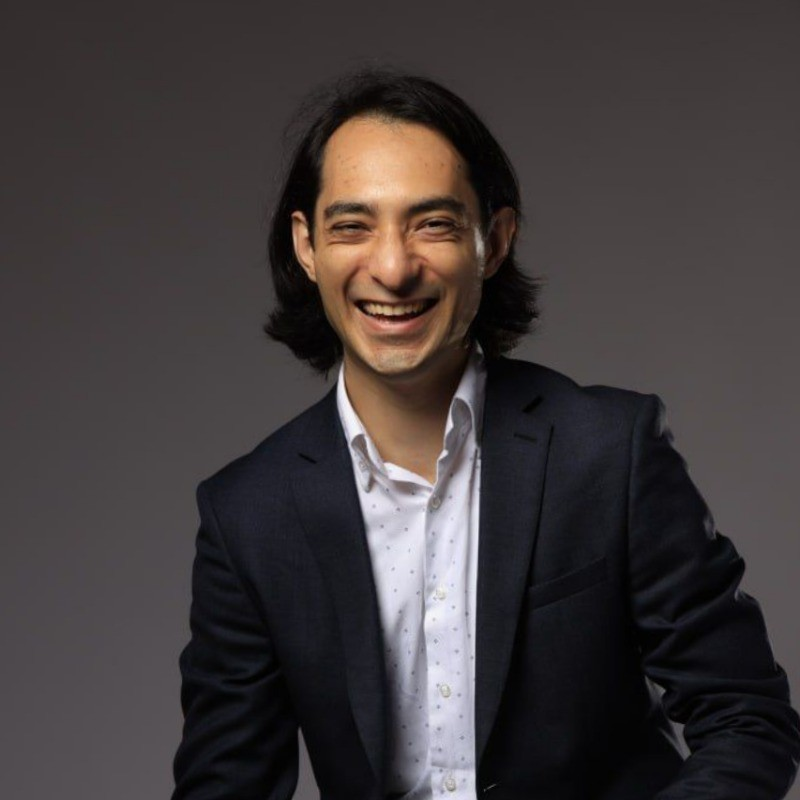
\includegraphics[width=3cm, height=3cm]{profile.jpeg}%
    };
  \end{tikzpicture}
\end{minipage}


%-----------SUMMARY--------------------------
% Keep this short, simple and straigth to point

\section{Data analytics enginee | Soon to be product analyst}
\small{
Doctoral candidate and data analytics engineer with six years of experience in academic and consultancy settings, where they built insight-driven dashboards, strong data models, and end-to-end data pipelines with carefully curated visualisations. I have extensive expertise developing ETL/ELT workflows and converting complicated datasets into understandable, practical insights for stakeholders. I have extensive experience working with teams from many departments to establish key performance indicators, provide data for decision-making, and implement analytics solutions that have a direct impact on strategy.
}
%--------------------------------------------

%--------------SKILLS------------------------
% Add or remove resumeSectionTypes according to your needs



%--------------Technical Skills
\section{Technical Skills}
\begin{tabular*}{\textwidth}{r@{\extracolsep{\fill}}lcr@{\extracolsep{\fill}}lcr@{\extracolsep{\fill}}lcr@{\extracolsep{\fill}}lcr@{\extracolsep{\fill}}l}
  \textbf{Python:}              & \textcolor{accent}{$\CIRCLE \CIRCLE \CIRCLE  $ }\WS{3/5,}& &
  \textbf{PostgreSQL:}          & \textcolor{accent}{$\CIRCLE \CIRCLE \CIRCLE  $ }\WS{3/5,}& &
  \textbf{DuckDB:}              & \textcolor{accent}{$\CIRCLE \CIRCLE \CIRCLE \CIRCLE $ }\WS{4/5,}& &
  \textbf{SQL:}                 & \textcolor{accent}{$\CIRCLE \CIRCLE \CIRCLE  $ }\WS{3/5,}& &
  \\
  
  \textbf{Spatial data:}        & \textcolor{accent}{$\CIRCLE \CIRCLE \CIRCLE \CIRCLE \CIRCLE$ }& &
  \textbf{LLM/NLP/LLM:}         & \textcolor{accent}{$\CIRCLE \CIRCLE \CIRCLE \CIRCLE $ }\WS{4/5,}& &
  \textbf{SQLite:}              & \textcolor{accent}{$\CIRCLE \CIRCLE \CIRCLE  $ }\WS{3/5,}& &
  \textbf{AZURE:}               & \textcolor{accent}{$\CIRCLE \CIRCLE   $ }\WS{2/5,}& &
  \\
  
  \textbf{GCP:}                 & \textcolor{accent}{$\CIRCLE \CIRCLE \CIRCLE \CIRCLE $ }\WS{4/5,}& &
  \textbf{R:}                   & \textcolor{accent}{$\CIRCLE \CIRCLE \CIRCLE \CIRCLE $ }\WS{4/5,} & &
  \textbf{MongoDB:}             & \textcolor{accent}{$\CIRCLE \CIRCLE   $ }\WS{2/5,}& &
  \textbf{Excel:}               & \textcolor{accent}{$\CIRCLE \CIRCLE \CIRCLE \CIRCLE $ }\WS{4/5,}& &
  \\
  
  \textbf{AcrGIS:}              & \textcolor{accent}{$\CIRCLE \CIRCLE \CIRCLE $ }\WS{3/5,}& &
  \textbf{ETL/ELT:}             & \textcolor{accent}{$\CIRCLE \CIRCLE \CIRCLE \CIRCLE $ }\WS{4/5,}& &
  \textbf{Cartography:}         & \textcolor{accent}{$\CIRCLE \CIRCLE \CIRCLE \CIRCLE $ }\WS{4/5,}& &
  \textbf{STATA:}               & \textcolor{accent}{$\CIRCLE \CIRCLE \CIRCLE \CIRCLE $ }\WS{4/5,}& &
  \\
  
  \textbf{Git:}                 & \textcolor{accent}{$\CIRCLE \CIRCLE \CIRCLE $ }\WS{3/5,}& &
  \textbf{RAG:}                 & \textcolor{accent}{$\CIRCLE \CIRCLE \CIRCLE \CIRCLE \CIRCLE$ }\WS{5/5,}& &
  \textbf{Julia:}               & \textcolor{accent}{$\CIRCLE \CIRCLE   $ }\WS{2/5,}& &
  \textbf{PowerBI:}             & \textcolor{accent}{$\CIRCLE \CIRCLE $ }\WS{2/5,}& &
  \\

\end{tabular*}

%--------------SOFT SKILLS
\section{Soft Skills}
\begin{tabular*}{\textwidth}{r@{\extracolsep{\fill}}lcr@{\extracolsep{\fill}}lcr@{\extracolsep{\fill}}lcr@{\extracolsep{\fill}}l}
  \textbf{Team work:}&            \textcolor{accent}{$\CIRCLE \CIRCLE \CIRCLE  $} \WS{3/5,}& &
  \textbf{Self-organised:}&       \textcolor{accent}{$\CIRCLE \CIRCLE \CIRCLE  $}\WS{3/5,} & &
  \textbf{Project management:}&   \textcolor{accent}{$\CIRCLE \CIRCLE \CIRCLE \CIRCLE $}\WS{4/5,}
  \\
  \textbf{Accounting:}&           \textcolor{accent}{$\CIRCLE \CIRCLE   $}\WS{2/5,} & &
  \textbf{Quality control:}&      \textcolor{accent}{$\CIRCLE \CIRCLE \CIRCLE \CIRCLE $}\WS{4/5,} & &
  \textbf{Visual communication:}& \textcolor{accent}{$\CIRCLE \CIRCLE \CIRCLE \CIRCLE \CIRCLE$} \WS{5/5,}
  \\
  \textbf{Quantiative research:}& \textcolor{accent}{$\CIRCLE \CIRCLE \CIRCLE \CIRCLE $}\WS{4/5,} & &
  \textbf{Prompt engineering:}&   \textcolor{accent}{$\CIRCLE \CIRCLE \CIRCLE \CIRCLE $}\WS{4/5,} & &
  \textbf{Document Management:}&  \textcolor{accent}{$\CIRCLE \CIRCLE \CIRCLE \CIRCLE $}\WS{4/5,} & &
  \\

\end{tabular*}


%----------------SKILLS----------------------





%  \section{Technical Skills}
%  
%  \resumeHeadingListStart{}
%  \resumeSectionType{Data Science}{:}{Time-series} \\
%  \resumeHeadingListEnd{}
%--------------------------------------------



%-----------EXPERIENCE-----------------------
% Distill all your talking points to small bullet points which follow the pattern "challenge-action-result" for maximum efficiency. Try to quantify (use numbers) your points whenver possible, highlist words of importance

\section{Experience}
\resumeHeadingListStart{}
\resumeQuadHeading{DATA ANALYTICS \& ENGINEERING}{Jan 2025 -- Present}
{Self-Employed | Consultant}{Project-Based -- Espoo, Finland}
Delivering end-to-end data engineering, analytics, and BI solutions tailored to each client's industry and business objectives. Advising on data strategy with a focus on scalability and sustainable growth.
As a data specialist, I design efficient pipelines that handle diverse data types and translate complex data into clear, actionable insights aligned with client goals.

\resumeQuadHeadingChild{Building Information Backend}{Jan 2026 -- Present}
{Apex-Heat -- Finland}
\resumeItemListStart{}
\resumeItem{Consulting on data transformation and business logic to facilitate future integration of spatial data with third-party systems.}
\resumeItem{Developing a data pipeline to transform and compute key metrics from building spatial data across Finland.}
\resumeItem{Designing and implementing an \textbf{API-based pipeline} for automated building calculations in Finland.}
\resumeItem{Evaluating and structuring spatial data models for EU-wide coverage.}
\resumeItem{Modelling data leveraging domain expertise in real estate economics and zoning regulations.}
\resumeItemListEnd{}

\resumeQuadHeadingChild{Optimisation \& Technical Debt Reduction}{Jan 2025 -- Dec 2025}
{Apex-Heat -- Finland}
\resumeItemListStart{}
\resumeItem{Identified and resolved \textbf{technical debt}, significantly improving data pipeline performance and maintainability.}
\resumeItem{Led migration from \textbf{Pandas} to \textbf{Polars} (including GeoPandas), reducing computation time and improving overall pipeline efficiency.}
\resumeItem{Refactored codebase design patterns and produced comprehensive \textbf{technical documentation}.}
\resumeItem{Expanded and improved \textbf{test coverage} and testing methodologies for data processing workflows.}
\resumeItemListEnd{}



\noindent\rule{0.5\linewidth}{0.4pt}
\pagebreak

% -------------------------------------------------------
\resumeQuadHeading{Ph.D. Candidate}{Sep 2020 -- Present}
{Aalto University}{Full-time -- Espoo, Finland}
Conducting doctoral research in urban and real estate economics, applying econometric and machine learning techniques to housing markets, real estate development, and urban planning. Managing the full spatial data lifecycle across research projects, from collection and processing to analysis and visualization, while building and maintaining the team's data infrastructure.

\resumeItemListStart{}
\resumeItem{Preparing and maintaining \textbf{data visualizations} for academic presentations and lectures.}
\resumeItem{Designing data-pipelines for local AI to extract features from text and scrctured data.}
\resumeItem{Providing IT service and assitance to my research team to resolve issues with their computers and software.}
\resumeItem{Applying Econometric, ML, time-series and data analysis for \textbf{quantitative research}.}
\resumeItem{Processing HTML and PDF files and implementing \textbf{RAG} to extract structured data from the land use plan documents.}
\resumeItem{Conducting \textbf{econometric} and \textbf{hedonic regression} analyses on property markets, housing development, and real estate dynamics.}
\resumeItem{Acquiring GIS data from REST and ArcGIS Online endpoints in the Netherlands to construct a longitudinal panel dataset for research.}
\resumeItem{Deploying and maintaining \textbf{Azure Functions} to automate web scraping of property listings and store real estate data for research purposes.}
\resumeItem{Performing \textbf{GIS analysis} to produce and maintain geospatial research datasets and geocode real estate transactions from data sources such as MML, Ryhti, SYKE, and KVKL.}
\resumeItem{Designing and deploying research databases using \textbf{PostgreSQL} and \textbf{DuckDB} to support team-wide data access.}
\resumeItem{Applying \textbf{time-to-event} statistical modelling, including longitudinal, repeating event, multi-state, and joint models.}
\resumeItem{Building and managing \textbf{ETL/ELT pipelines} with data stewardship responsibilities to acquire, curate, and distribute research datasets.}

\resumeItemListEnd{}


\resumeQuadHeadingChild{Research Assistant}{Jun 2019 -- Sep 2019}
{Aalto University}{Full-time -- Espoo, Finland}
Contributed to an \textbf{Agent-Based Modelling (ABM)} research project simulating urban mobility and parking pressure, developed in collaboration with \textbf{MIT CityLab}.

\resumeItemListStart{}
\resumeItem{Developed an \textbf{ABM simulation} to model parking pressure dynamics in the Otaniemi campus area.}
\resumeItem{Collaborated with \textbf{MIT CityLab} on agent-based modelling of urban mobility patterns.}
\resumeItem{Implemented simulations using the \textbf{GAMA Platform}.}
\resumeItemListEnd{}
\noindent\rule{0.5\linewidth}{0.4pt}


% ------------------------------------------------------------------------------

\resumeQuadHeading{Data Analytics Engineer}{Sep 2020 -- Dec 2024}
{Qissa kaupunkisuunnitteluanalytiikka Oy -- Startup}{Part-time -- Espoo, Finland}

Delivered data engineering and spatial analysis solutions for an urban analytics startup, supporting clients in urban planning and sustainability with end-to-end data workflows.

\resumeItemListStart{}
\resumeItem{Designed and maintained data pipelines to ingest \textbf{GIS data} from REST APIs, performing cleaning, \textbf{geocoding}, and storage in line with client specifications.}
\resumeItem{Built a \textbf{spatial analytics dashboard} with a network analysis backend, integrating \textbf{HSL, HERE, and HSY APIs} to gather, process, and perform \textbf{spatial network analysis}.}
\resumeItem{Extracted, processed, and served \textbf{census data} from the US, Denmark, Sweden, and Finland to calculate CO\textsubscript{2} emissions from commuting patterns.}
\resumeItemListEnd{}
\noindent\rule{0.5\linewidth}{0.4pt}

% ------------------------------------------------------------------------------

\resumeQuadHeading{Planning Assistant}{Nov 2018 -- Jun 2021}
{WSP Finland Oy}{Part-time -- Helsinki, Finland}

Provided GIS and spatial data analysis support across urban planning and transport projects, delivering actionable insights and visualizations to multidisciplinary teams and external clients.

\resumeItemListStart{}
\resumeItem{Conducted \textbf{spatial data analysis}, processing and managing geospatial datasets across multiple concurrent projects.}
\resumeItem{Performed \textbf{pedestrian network analysis} to forecast route choice and model post-development pedestrian flows, calibrated against real-world conditions.}
\resumeItem{Prepared maps, graphs, and \textbf{data visualizations} for stakeholders, project managers, and clients to support planning decisions.}
\resumeItem{Delivered \textbf{GIS analysis} to cross-disciplinary teams including transport engineers, landscape designers, urban planners, and architects.}
\resumeItem{Configured \textbf{ArcGIS Online} platforms to support \textbf{maritime spatial planning} workflows.}
\resumeItem{Developed dynamic \textbf{3D city models} using \textbf{ESRI CityEngine} to visualize urban development scenarios.}
\resumeItemListEnd{}
\noindent\rule{0.5\linewidth}{0.4pt}
% ------------------------------------------------------------------------------

\resumeQuadHeading{GIS Operator}{Aug 2015 -- May 2016}
{University of Tehran}{Part-time -- Tehran, Iran}
\resumeItemListStart{}
\resumeItem{Collected, processed, and prepared \textbf{GIS datasets} to support urban designers in implementing and evaluating new urban design directives for Tehran.}
\resumeItemListEnd{}
\noindent\rule{0.5\linewidth}{0.4pt}

% \resumeQuadHeading{Advisor \& Assistant}{Aug 2011 -- Aug 2018}
% {Airsa Dorsa Co. Ltd. -- Family Business}{Full-time -- Karaj, Iran}
% Led day-to-day operations of a manufacturing business, overseeing financial management, client relations, production coordination, and technical delivery across a broad range of functions.

% \resumeItemListStart{}
% \resumeItem{Managed \textbf{accounting}, cost calculations, financial analysis, and HR processes, producing BI reports to support business decisions.}
% \resumeItem{Delivered in-house \textbf{graphic design}, CAD drafting, and technical solutions tailored to client requirements.}
% \resumeItem{Negotiated with clients on designs, pricing, and production specifications to ensure alignment and satisfaction.}
% \resumeItem{Coordinated and tracked production timelines, maintenance schedules, and order delivery to meet deadlines.}
% \resumeItem{Conducted auditing, inventory management, and process oversight to maintain operational efficiency.}
% \resumeItem{Performed hands-on technical duties including supervision, high-frequency welding, and silk screen printing.}
% \resumeItemListEnd{}
%---------------------------------------------



\resumeHeadingListEnd{}
%---------------------------------------------
\section{Machine Learning $|$ Statistical models $|$ Econometrics}
\begin{tabular*}{\textwidth}{r@{\extracolsep{\fill}}lcr@{\extracolsep{\fill}}lcr@{\extracolsep{\fill}}lcr@{\extracolsep{\fill}}l}
  \textbf{Uni-variate time-series:}& \textcolor{accent}{$\CIRCLE \CIRCLE \CIRCLE$} \WS{3/5,}& &
  \textbf{VAR time-series:}& \textcolor{accent}{$\CIRCLE \CIRCLE \CIRCLE  $} \WS{3/5,}& &
  \textbf{Co-integration time-series:}& \textcolor{accent}{$\CIRCLE \CIRCLE   $} \WS{2/5,}& &
  \\
  \textbf{multi-variate time-series:}& \textcolor{accent}{$\CIRCLE \CIRCLE \CIRCLE  $} \WS{3/5,}& &
  \textbf{OLS:}& \textcolor{accent}{$\CIRCLE \CIRCLE \CIRCLE \CIRCLE \CIRCLE$} \WS{5/5,}& &
  \textbf{IV-OLS:}& \textcolor{accent}{$\CIRCLE \CIRCLE \CIRCLE \CIRCLE $} \WS{4/5,}& &
  \\
  \textbf{Panel data:}& \textcolor{accent}{$\CIRCLE \CIRCLE \CIRCLE \CIRCLE $} \WS{4/5,}& &
  \textbf{Generalised Method of Moments:}& \textcolor{accent}{$\CIRCLE \CIRCLE \CIRCLE \CIRCLE $} \WS{4/5,}& &
  \textbf{Generalised linear models:}& \textcolor{accent}{$\CIRCLE \CIRCLE $} \WS{2/5,}& &
  \\
  \textbf{Spatial econometrics:}& \textcolor{accent}{$\CIRCLE \CIRCLE \CIRCLE \CIRCLE $} \WS{4/5,}& &
  \textbf{Survival/time-to-event:}& \textcolor{accent}{$\CIRCLE \CIRCLE \CIRCLE \CIRCLE \CIRCLE$} \WS{5/5,}& &
  \textbf{Additive hazard models:}& \textcolor{accent}{$\CIRCLE \CIRCLE \CIRCLE \CIRCLE \CIRCLE$} \WS{5/5,}& &
  \\

\end{tabular*}

%-----------EDUCATION-------------------------
% Mention your CGPA, if its good, in the first row of second column

\section{Education}

\resumeHeadingListStart{}
\resumeQuadHeading{Aalto University}{Espoo, Finland}
{Doctor of Philosophy in Technology, Real Estate Economics}{Sep 2020 - Present}
\resumeHeadingListEnd{}

\resumeHeadingListStart{}
\resumeQuadHeading{Aalto University}{Espoo, Finland}
{MSc. (Tech.) Urban Studies and Planning in Real Estate Economic}{Sep 2018 - Jul 2020}
GPA: 4.1/5, Graduated with honours
\resumeHeadingListEnd{}

\resumeHeadingListStart{}
\resumeQuadHeading{University of Tehran}{Tehran, Iran}
{BA. Town Planning}{Sep 2011 - Jun 2015}
GPA: 16.67/20, Academic excellence
\resumeHeadingListEnd{}
%---------------------------------------------


%-----------PROJECTS--------------------------
% Use resumeQuadHeading if four elements are feasible (ex: demo video link), else use resumeTrioHeading. Keep the bullet points simple and concise and try to cover wide variety of skills you have used to build these projects

%  \section{Projects}
%  \resumeHeadingListStart{}
%  \resumeTrioHeading{\href{https://project1.com}{\uline{Project 1}}}{React.js, Redux, PHP, MySQL Git}{\href{https://proect1.com/source-code/}{\uline{Source Code}}}
%  \resumeItemListStart{}
%  \resumeItem{Designed and developed a clean and modern website using \textbf{HTML, CSS, and JavaScript}}
%  \resumeItem{Optimized website for \textbf{speed and user experience}}
%  \resumeItem{Utilized \textbf{responsive design} to ensure compatibility across all devices}
%  \resumeItem{Deployed on GitHub pages via GitHub Actions}
%  \resumeItemListEnd{}
%  
%  \resumeTrioHeading{Project 2}{Node.js, Express, JavaScript, Git}{\href{https:project2.com/source-code}{\uline{Source Code}}}
%  \resumeItemListStart{}
%  \resumeItem{A \textbf{CRUD application} exposed using a RESTful API made with Node.js}
%  \resumeItem{Exposed POST, GET, PATCH and DELETE HTTP methods using \textbf{Express}}
%  \resumeItemListEnd{}
%  \resumeHeadingListEnd{}
%--------------------------------------------




%----------------OTHERS----------------------
% You can add your acheivements, accolades, certifications etc. here.

\section{Volunteer Work}
\resumeItemListStart{}
\resumeItem{DataTribe collective moderator, contributor}
\resumeItem{DataTribe collective speaker: Spatial data analysis, spatial data engineering}
\resumeItem{Helsinki Data Week volunteer (2024 \& 2025), contributor}

\resumeItemListEnd{}
%--------------------------------------------

\vfill
\textit {Disclaimer: This resume is designed with \LaTeX, and contains white text for the skill ratings to increase the accuracy of automated scanning and processing.}

\end{document}